\subsection{Resolved Issues} \label{subsec:spr1_resolved_issues}

\begin{longtable} { | c | p{12cm} | c | } 
\hline
	ID 	&	Issue	&		 Es. hours \\\hline
	6	& 	Changing application name	&	1 hour	\\\hline
\caption{Issue ID 6}
\label{tab:spr1_issue6}
\end{longtable}
This was a trivial task of changing the application name in the AndroidManifest of the project. The project is as mentioned now called Sekvens as opposed to the former name Zebra. The change was made due to one of the very first customer requests; the applications within GIRAF should have eloquent names, rather than names from the earlier savannah animal theme.

\begin{longtable} { | c | p{12cm} | c | } 
\hline
	ID 	&	Issue	&		 Es. hours \\\hline
	10	& 	Changing a sequence name is not intuitive	&	8 hours	\\\hline
\caption{Issue ID 10}
\label{tab:spr1_issue10}
\end{longtable}
Changing the name of a sequence was previously done by clicking on the title text, but it was not obvious that it was in fact editable.  The issue was resolved by adding a button (as shown in figure \ref{fig:Old_editName}) which programmatic places the cursor in the textfield and popping up the virtual keyboard. We felt like this cluttered the entire GUI with too many buttons, so we decided to keep the issue open for later revision. No icons displays editing the name therefore we used a simple white placeholder with the word `TEXT' on it. 
\begin{figure} [h!]
\centering
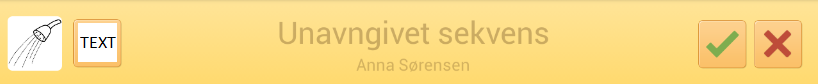
\includegraphics[width=0.8\textwidth]{Pics/Sprint1/editName/editNameButton.png}
\caption{This is a picture of top bar after the edit button was added}
\label{fig:Old_editName}
\end{figure}

\begin{longtable} { | c | p{12cm} | c | } 
\hline
	ID 	&	Issue	&		 Es. hours \\\hline
	11	& 	Analyzing TODOs in code	&	16 hours	\\\hline
	17	& 	Solve TODO in SequenceViewGroup - Can child be bigger than parent?	&	2 hours	\\\hline
\caption{Issue ID 11 and 17}
\label{tab:spr1_issues11_17}
\end{longtable}

Solving the TODO's of the previous group who worked on the project was one of the more difficult issues. They were usually very unclear, examples being \ct{//TODO: ???} and \ct{//TODO: this is ridiculous}. Since statements were this vague and seemingly not meant for other groups to understand, these issues were time consuming. The estimate of 16 hours however fit surprisingly well for both analyzing and solving the issues. This is partly due to some of the previous groups lack of understanding for Android programming. These TODO's could thus just be removed. Issue 17 was created as a separate task because it was difficult to troubleshoot, but it was found to that code already existed to ensure that a child view could not be bigger than the parent view.

\begin{longtable} { | c | p{12cm} | c | } 
\hline
	ID 	&	Issue	&		 Es. hours \\\hline
	14	& 	Import temporary pictures into Sequence	&	4 hours	\\\hline
\caption{Issue ID 14}
\label{tab:spr1_issue14}
\end{longtable}
While Sekvens was runnable from the beginning of the sprint, it had no pictograms available. This did not change during sprint 1. Therefore, having some local images to use in the application would be beneficial. It was discovered that one of the previous groups had hardcoded paths and names for pictograms that we had no access to. Pasting new images with matching titles on the hardcoded path allowed us to have images to work with in the application.

\begin{longtable} { | c | p{12cm} | c | } 
\hline
	ID 	&	Issue	&		 Es. hours \\\hline
	18	& 	Child selected upon opening the program is not highlighted	&	2 hours	\\\hline
\caption{Issue ID 18}
\label{tab:spr1_issue18}
\end{longtable}
This issue was looked into but turned out to be difficult to solve. However, while it was in fact never fixed, it also became a non-issue due to new requirements. These requirements specified that the child list should not be available from within Sekvens. Choosing children should be done from the Launcher application. The issue was therefore closed.

\begin{longtable} { | c | p{12cm} | c | } 
\hline
	ID 	&	Issues	&		 Es. hours \\\hline
	19	& 	Zebra is installed with two app-icons	&	16 hours	\\\hline
\caption{Issue ID 19}
\label{tab:spr1_issue19}
\end{longtable}
Debugging why the application was installed twice upon compiling was another hard issue. This was one of the first issues we attempted to solve, and lack of knowledge about Android made this simple fix a time-wise underestimated issue. We did not immediately realize that the issue was not within Sekvens, but in one of its dependencies. Once discovering the cause it was a simple fix of removing one line from a submodules Android Manifest.

\begin{longtable} { | c | p{12cm} | c | } 
\hline
	ID 	&	Issue	&		 Es. hours \\\hline
	20	& 	When a sequences is created it should have a return to overview button	&	8 hours	\\\hline
\caption{Issue ID 20}
\label{tab:spr1_issue20}
\end{longtable}
When displaying a created sequence it was not apparent how the user was able to return to the overview. The former way was by pressing the tablets back button, but it seemed rather unintuitive as it was supposed to go to the overview, and not back to editing the sequence. This was solved by adding a button to allow the user to return and furthermore overriding the tablets button to return to overview (A picture of the button is displayed in figure \ref{fig:Old_backButton}).
\begin{figure} [h!]
\centering

\includegraphics{Pics/Sprint1/Gammelt/back_button}
\caption{A picture of a simple button in `Sekvens'}
\label{fig:Old_backButton}
\end{figure} 